\chapter{ESG Preferences}

\section{Expected Utility and Optimal Portfolio}


\subsection{Setting the Investor's Expected Utility}

Let's assume a single period model, from $t=0$ to $t=1$.
We have $N$ stocks. 

We have a $N \times 1$ vector of returns $\tilde{r}_1$ at period 1, 
assumed to be normally distributed: 

\begin{equation}
    \tilde{r}_1 = \mu + \tilde{\epsilon}_1
\end{equation}

with $\mu$ the equilibrium expected excess returns and $\tilde{\epsilon}_1$ the
random component of the returns $\tilde{\epsilon}_1 \sim N(0, \Sigma)$.

The investor $i$ has an exponential CARA utility function, with 
$\tilde{W}_{1,i}$ the wealth at period 1, and $X_i$ the
$N \times 1$ vector of portfolio weights.

\begin{equation}
    V(\tilde{W}_{1,i}, X_i) = -\exp{(-A_i \tilde{W}_{1,i}-b_i^T X_i)}
\end{equation}

with $A_i$ agent's absolute risk aversion, $b_i$ an $N \times 1$ vector of nonpecuniary 
benefits. 

\begin{equation}
    b_i = d_i g 
\end{equation}

with $g$ an $N \times 1$ vector and $d_i \geq 0$ a scalar measuring 
the agent's taste for the nonpecuniary benefits.


The expectation of agent $i$'s in period 0 are:

\begin{equation}
    E_0(V(\tilde{W}_{1,i}, X_i)) = E_0(-\exp{(-A_i \tilde{W}_{1,i}-b_i^T X_i)})
\end{equation}

We can replace $\tilde{W}_{1,i}$ by the relation 
$\tilde{W}_{1,i} = W_{0,i}(1 + r_f + X_i^T \tilde{r}_1)$
 and define $a_i := A_i W_{0,i}$. The idea is to make out from the
expectation the terms that we know about (in period 0), and reexpress 
the terms within the expectation as a function of the
portfolio weights $X_i$. The last two steps use the fact that 
$\tilde{r}_1$ is normally distributed with mean $\mu$ and variance $\Sigma$.

\begin{equation}
    \begin{aligned}
    E_0(V(\tilde{W}_{1,i}, X_i)) = E_0(-\exp{(-A_i W_{0,i}(1 + r_f + X_i^T \tilde{r}_1)-b_i^T X_i)}) \\
    = E_0(-\exp{(-a_i(1 + r_f + X_i^T \tilde{r}_1)-b_i^T X_i)})  \\
    = E_0(-\exp{(-a_i(1 + r_f) - a_i X_i^T \tilde{r}_1 - b_i^T X_i)}) \\
    = -\exp{(-a_i(1 + r_f))} E_0(-\exp{(-a_i X_i^T \tilde{r}_1 - b_i^T X_i)}) \\
    = -\exp{(-a_i(1 + r_f))} E_0(-\exp{(-a_i X_i^T (\tilde{r}_1 + \frac{b_i}{a_i}))})  \\
    = -\exp{(-a_i (1 + r_f))} \exp{(-a_i X_i^T (E_0(\tilde{r}_1) + \frac{b_i}{a_i})+\frac{1}{2}a_i^2 X_i^T \text{Var}(\tilde{r}_1)X_i)} \\
    = -\exp{(-a_i (1 + r_f))} \exp{(-a_i X_i^T (\mu + \frac{b_i}{a_i})+\frac{1}{2}a_i^2 X_i^T \Sigma X_i)} \\
    \end{aligned}
\end{equation}

\subsection{Solving for the Investor's Optimal Portfolio}

The investors choose their optimal portfolios at time 0. 
The optimal portfolio $X_i$ is the one that maximizes the expected utility.
To find it, we differentiate the expected utility with respect to $X_i$ and 
set it to zero, to obtain the first-order condition.

We are going to do it step by step:

\begin{enumerate}
    \item Combine the Exponential Terms:
    \begin{equation}
        E_0(V(\tilde{W}_{1,i}, X_i)) = -\exp{(-a_i(1 + r_f)-a_iX_i^T(\mu + \frac{b_i}{a_i})+\frac{1}{2}a_i^2X_i^T\Sigma X_i)}
    \end{equation}
    and let $f(X_i)$ be the exponent:
    \begin{equation}
        E_0(V(\tilde{W}_{1,i}, X_i)) = -\exp{f(X_i)}
    \end{equation}
    \item Differentiate $f(X_i)$ with respect to $X_i$. We have the 
    chain rule:
    \begin{equation}
        \frac{\partial h}{\partial X_i} = \frac{\partial h}{\partial f} \frac{\partial f}{\partial X_i}
    \end{equation}
    If $h = - \exp{(f)}$, then $\frac{\partial h}{\partial f} = - \exp{(f)}$. 
    Therefore we have:
    \begin{equation}
        \frac{\partial h}{\partial X_i} = -\exp{(f)} \frac{\partial f}{\partial X_i}
    \end{equation}
    To tackle the derivative of $f(X_i)$, we use two rules. First $\frac{\partial x^T b}{\partial x} = b$ and
    $\frac{\partial x^T A x}{\partial x} = 2Ax$ if $A$ is symmetric. We have:
    \begin{equation}
        \frac{\partial f}{\partial X_i} = -a_i(\mu + \frac{b_i}{a_i}) + a_i^2 \Sigma X_i
    \end{equation}
    Combining:
    \begin{equation}
        \frac{\partial h}{\partial X_i} = -\exp{(f)} ( -a_i(\mu + \frac{b_i}{a_i}) + a_i^2 \Sigma X_i)
    \end{equation}
    \item Set the derivative to zero:
    \begin{equation}
        \begin{aligned}
            -\exp{(f)} ( -a_i(\mu + \frac{b_i}{a_i}) + a_i^2 \Sigma X_i) = 0 \\
            -a_i(\mu + \frac{b_i}{a_i}) + a_i^2 \Sigma X_i = 0
        \end{aligned}
    \end{equation}
    where the exponential term is always positive, so we can drop it.
    \item Rearrange and solve for $X_i$:
    \begin{equation}
        \begin{aligned}
            a_i^2 \Sigma X_i = a_i(\mu + \frac{b_i}{a_i}) \\
            a_i \Sigma X_i = \mu + \frac{b_i}{a_i} \\
            \Sigma X_i = \frac{1}{a_i}( \mu + \frac{b_i}{a_i}) \\
            X_i = \frac{1}{a_i} \Sigma^{-1}(\mu + \frac{b_i}{a_i})
        \end{aligned}
    \end{equation}
\end{enumerate}


For the sake of simplicity, we assume that $a_i = a$ for all investors.
We now have:

\begin{equation}
    \begin{aligned}
    X_i = \frac{1}{a} \Sigma^{-1}(\mu + \frac{b_i}{a}) \\
    = \frac{1}{a} \Sigma^{-1}(\mu + \frac{d_i}{a}g) \\
    \end{aligned}
\end{equation}

Therefore, the optimal portfolio differs across investors due to the
ESG characteristics $g$ of the stocks and the investors' taste for
nonpecuniary benefits $d_i$. 


\begin{figure}
    \centering
    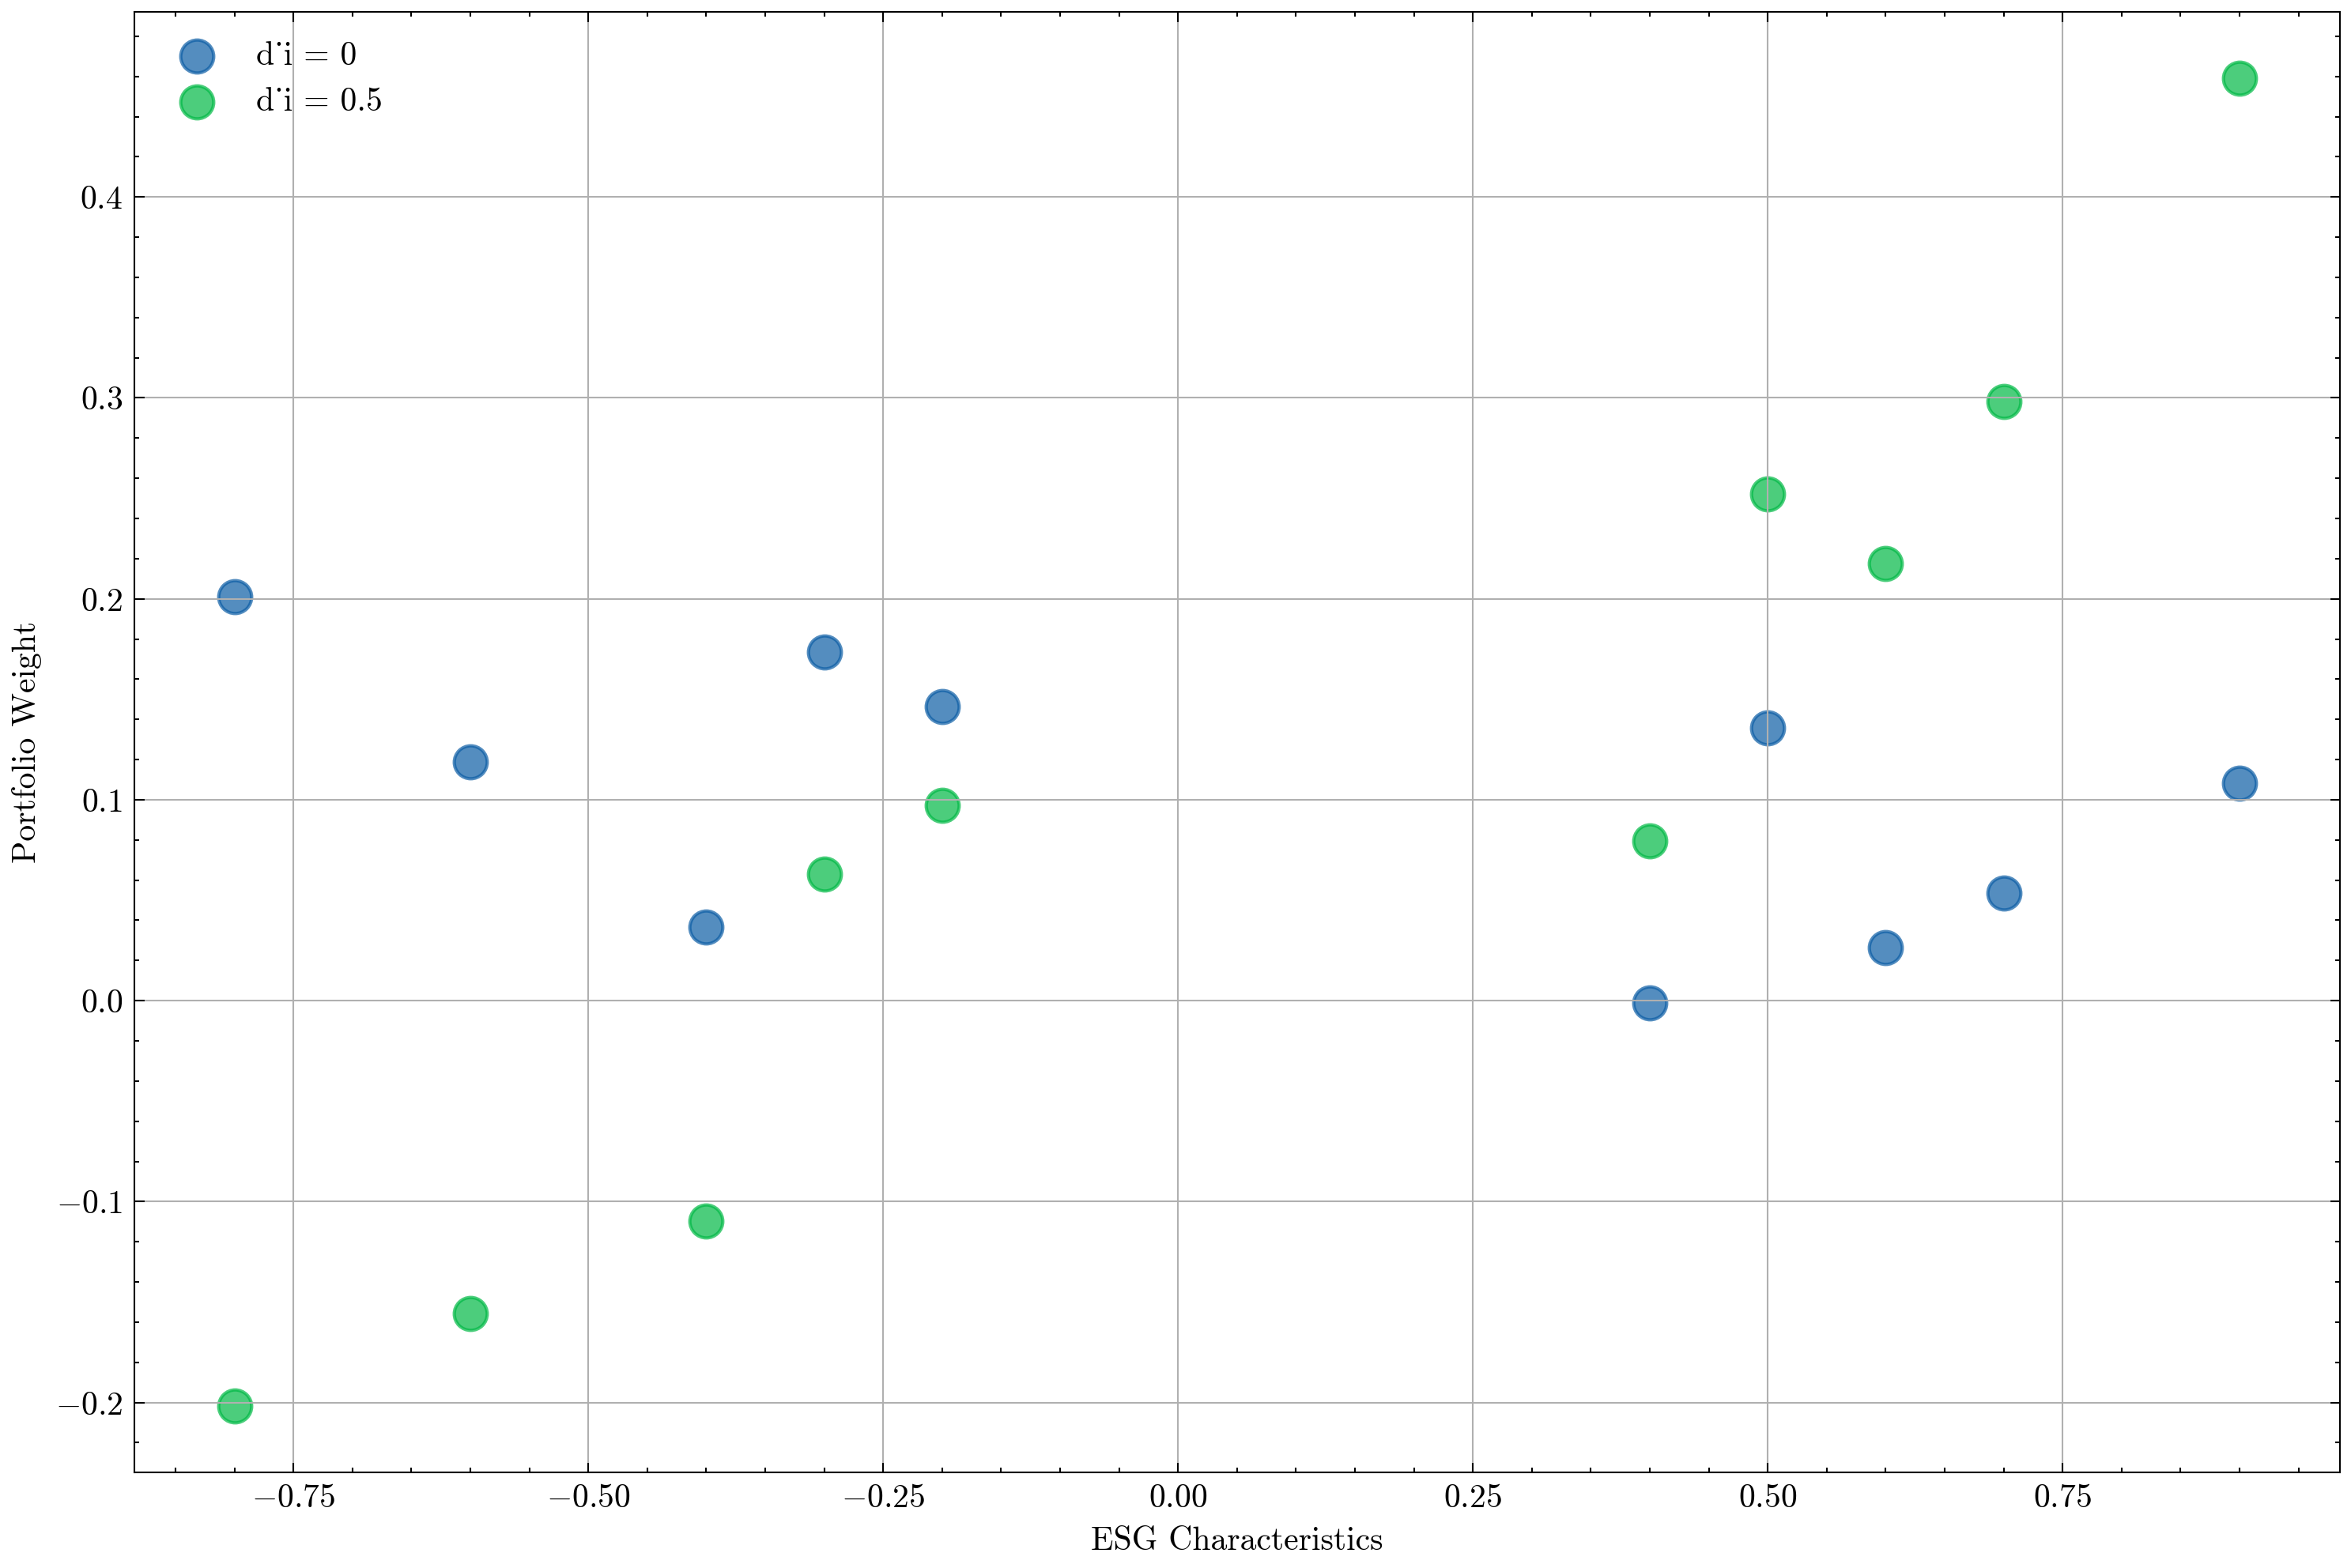
\includegraphics[width=1\textwidth]{../images/chapter01/portfolio_weights_vs_esg.png}
    \caption{Portfolio Weights vs ESG Preferences}
    \label{fig:esg_taste}
\end{figure}

\newpage

\section{Heterogeneous Investors and Expected Returns}


\subsection{Heterogeneous Market and Market Portfolio Weights}

The $n$th element of investor $i$'s portfolio weight vector $X_i$ is:

\begin{equation}
    X_{i,n} = \frac{W_{0,i,n}}{W_{0,i}}
\end{equation}

with $W_{0,i,n}$ the wealth invested in stock $n$ by investor $i$ at time 0.

The total wealth invested in stock $n$ at time 0 is:

\begin{equation}
    W_{0,n} := \int_i W_{0,i,n} di
\end{equation}

The $n$th element of the market-weight vector $w_m$ is:

\begin{equation}
    \begin{aligned}
    w_{m,n} = \frac{W_{0,n}}{W_{0}} \\
    \end{aligned}
\end{equation}

We can now express $W_{0,n}$ in terms of individual investors' wealths
by using the definition of $W_{0,n}$:

\begin{equation}
    w_{m,n} = \frac{1}{W_0} \int_i W_{0,i,n} di
\end{equation}

We now that $W_{0,i,n} = W_{0,i} X_{i,n}$, so we can rewrite the equation:

\begin{equation}
    w_{m,n} = \frac{1}{W_0} \int_i W_{0,i} X_{i,n} di
\end{equation}

Defining $\omega_i = \frac{W_{0,i}}{W_0}$, we have:

\begin{equation}
    \begin{aligned}
    w_{m,n} = \int_i \frac{W_{0,i}}{W_0} X_{i,n} di\\
    = \int_i \omega_i X_{i,n} di
    \end{aligned}
\end{equation}

We can now plug in $X_i$ to obtain $w_m$ the vector 
of market weights: 

\begin{equation}
    \begin{aligned}
    w_{m} = \int_i \omega_i X_i di \\ 
     = \int_i \omega_i \frac{1}{a} \Sigma^{-1}(\mu + \frac{d_i}{a}g)_n di \\
     = \frac{1}{a} \sigma^{-1} \mu (\int_i \omega_i di) + \frac{1}{a^2} \Sigma^{-1} g (\int_i \omega_i d_i di)
    \end{aligned}
\end{equation}


We have $\int_i \omega_i di = 1$ and we define $\bar{d} := \int_i d_i di \geq 0$,
the wealth-weighted mean of ESG tastes $d_i$ across agents. Therefore,
the market portfolio weights are:

\begin{equation}
    w_m = \frac{1}{a} \Sigma^{-1} \mu + \frac{1}{a^2} \Sigma^{-1} g \bar{d}
\end{equation}


\begin{figure}
    \centering
    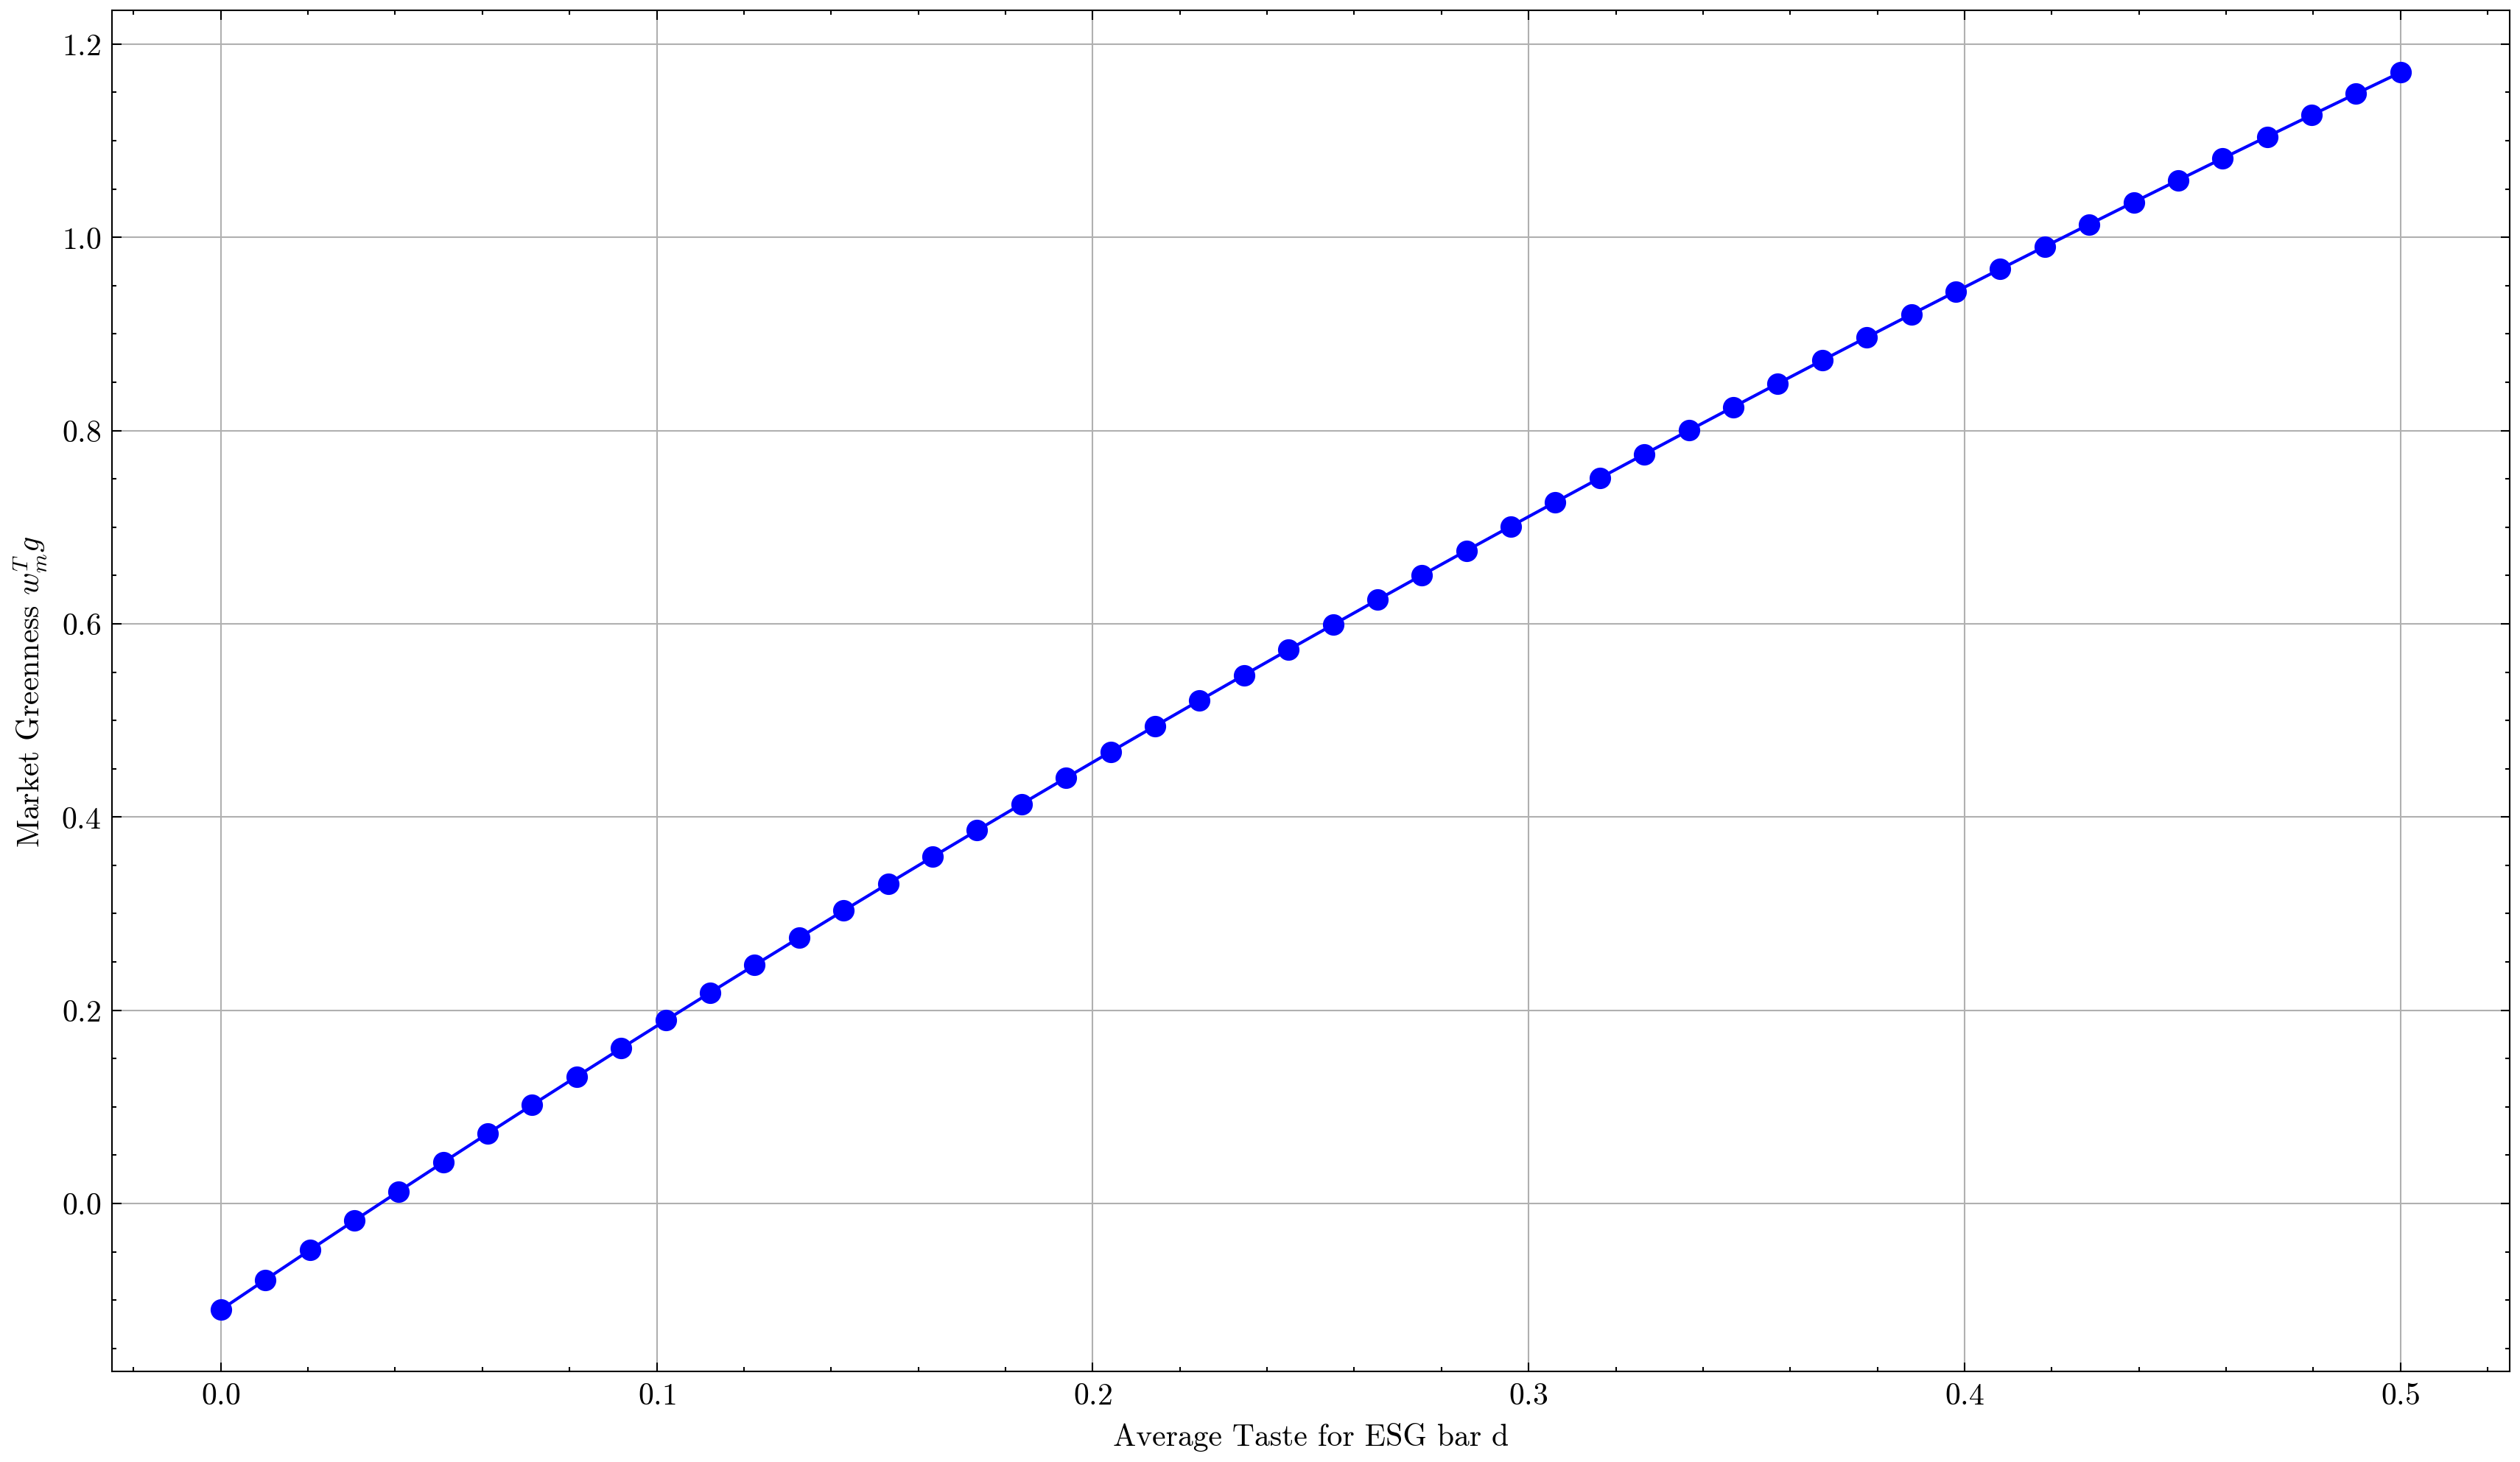
\includegraphics[width=1\textwidth]{../images/chapter01/market_greenness_vs_average_esg_taste.png}
    \caption{Relationship between Market Greenness and Average Taste for ESG}
    \label{fig:esg_taste_market}
\end{figure}

This equation is the same as the one found 
for the investor's optimal portfolio weights, but with the
average ESG tastes $\bar{d}$ instead of individual tastes $d_i$.

\subsection{Expected Returns}

Starting from the the vector of market weights $w_m$, we now can 
solve for $\mu$ the vector of expected returns. We have:

\begin{equation}
    \begin{aligned}
    w_m = \frac{1}{a} \Sigma^{-1} \mu + \frac{1}{a^2} \Sigma^{-1} g \bar{d} \\
    a w_m = \Sigma^{-1} \mu + \frac{1}{a} \Sigma^{-1} g \bar{d} \\
    a w_m - \frac{1}{a} \Sigma^{-1} g \bar{d} = \Sigma^{-1} \mu \\
    \Sigma (a w_m - \frac{1}{a} \Sigma^{-1} g \bar{d}) = \mu \\ 
    \mu = a \Sigma w_m - \frac{1}{a} \Sigma \Sigma^{-1} g \bar{d} \\
    \mu = a \Sigma w_m - \frac{1}{a} g \bar{d}
    \end{aligned}
\end{equation}

Multiplying by $w_m$, we find the market equity premium $\mu_m = w_m^T \mu$:

\begin{equation}
    \begin{aligned}
    \mu_m = a w_m^T \Sigma w_m - \frac{\bar{d}}{a} w_m^T g  \\
    = a \sigma_m^2 - \frac{\bar{d}}{a} w_m^T g 
    \end{aligned}
\end{equation}

where $\sigma_m^2 = w_m^T \Sigma w_m$ is the market return variance. 

\begin{figure}
    \centering
    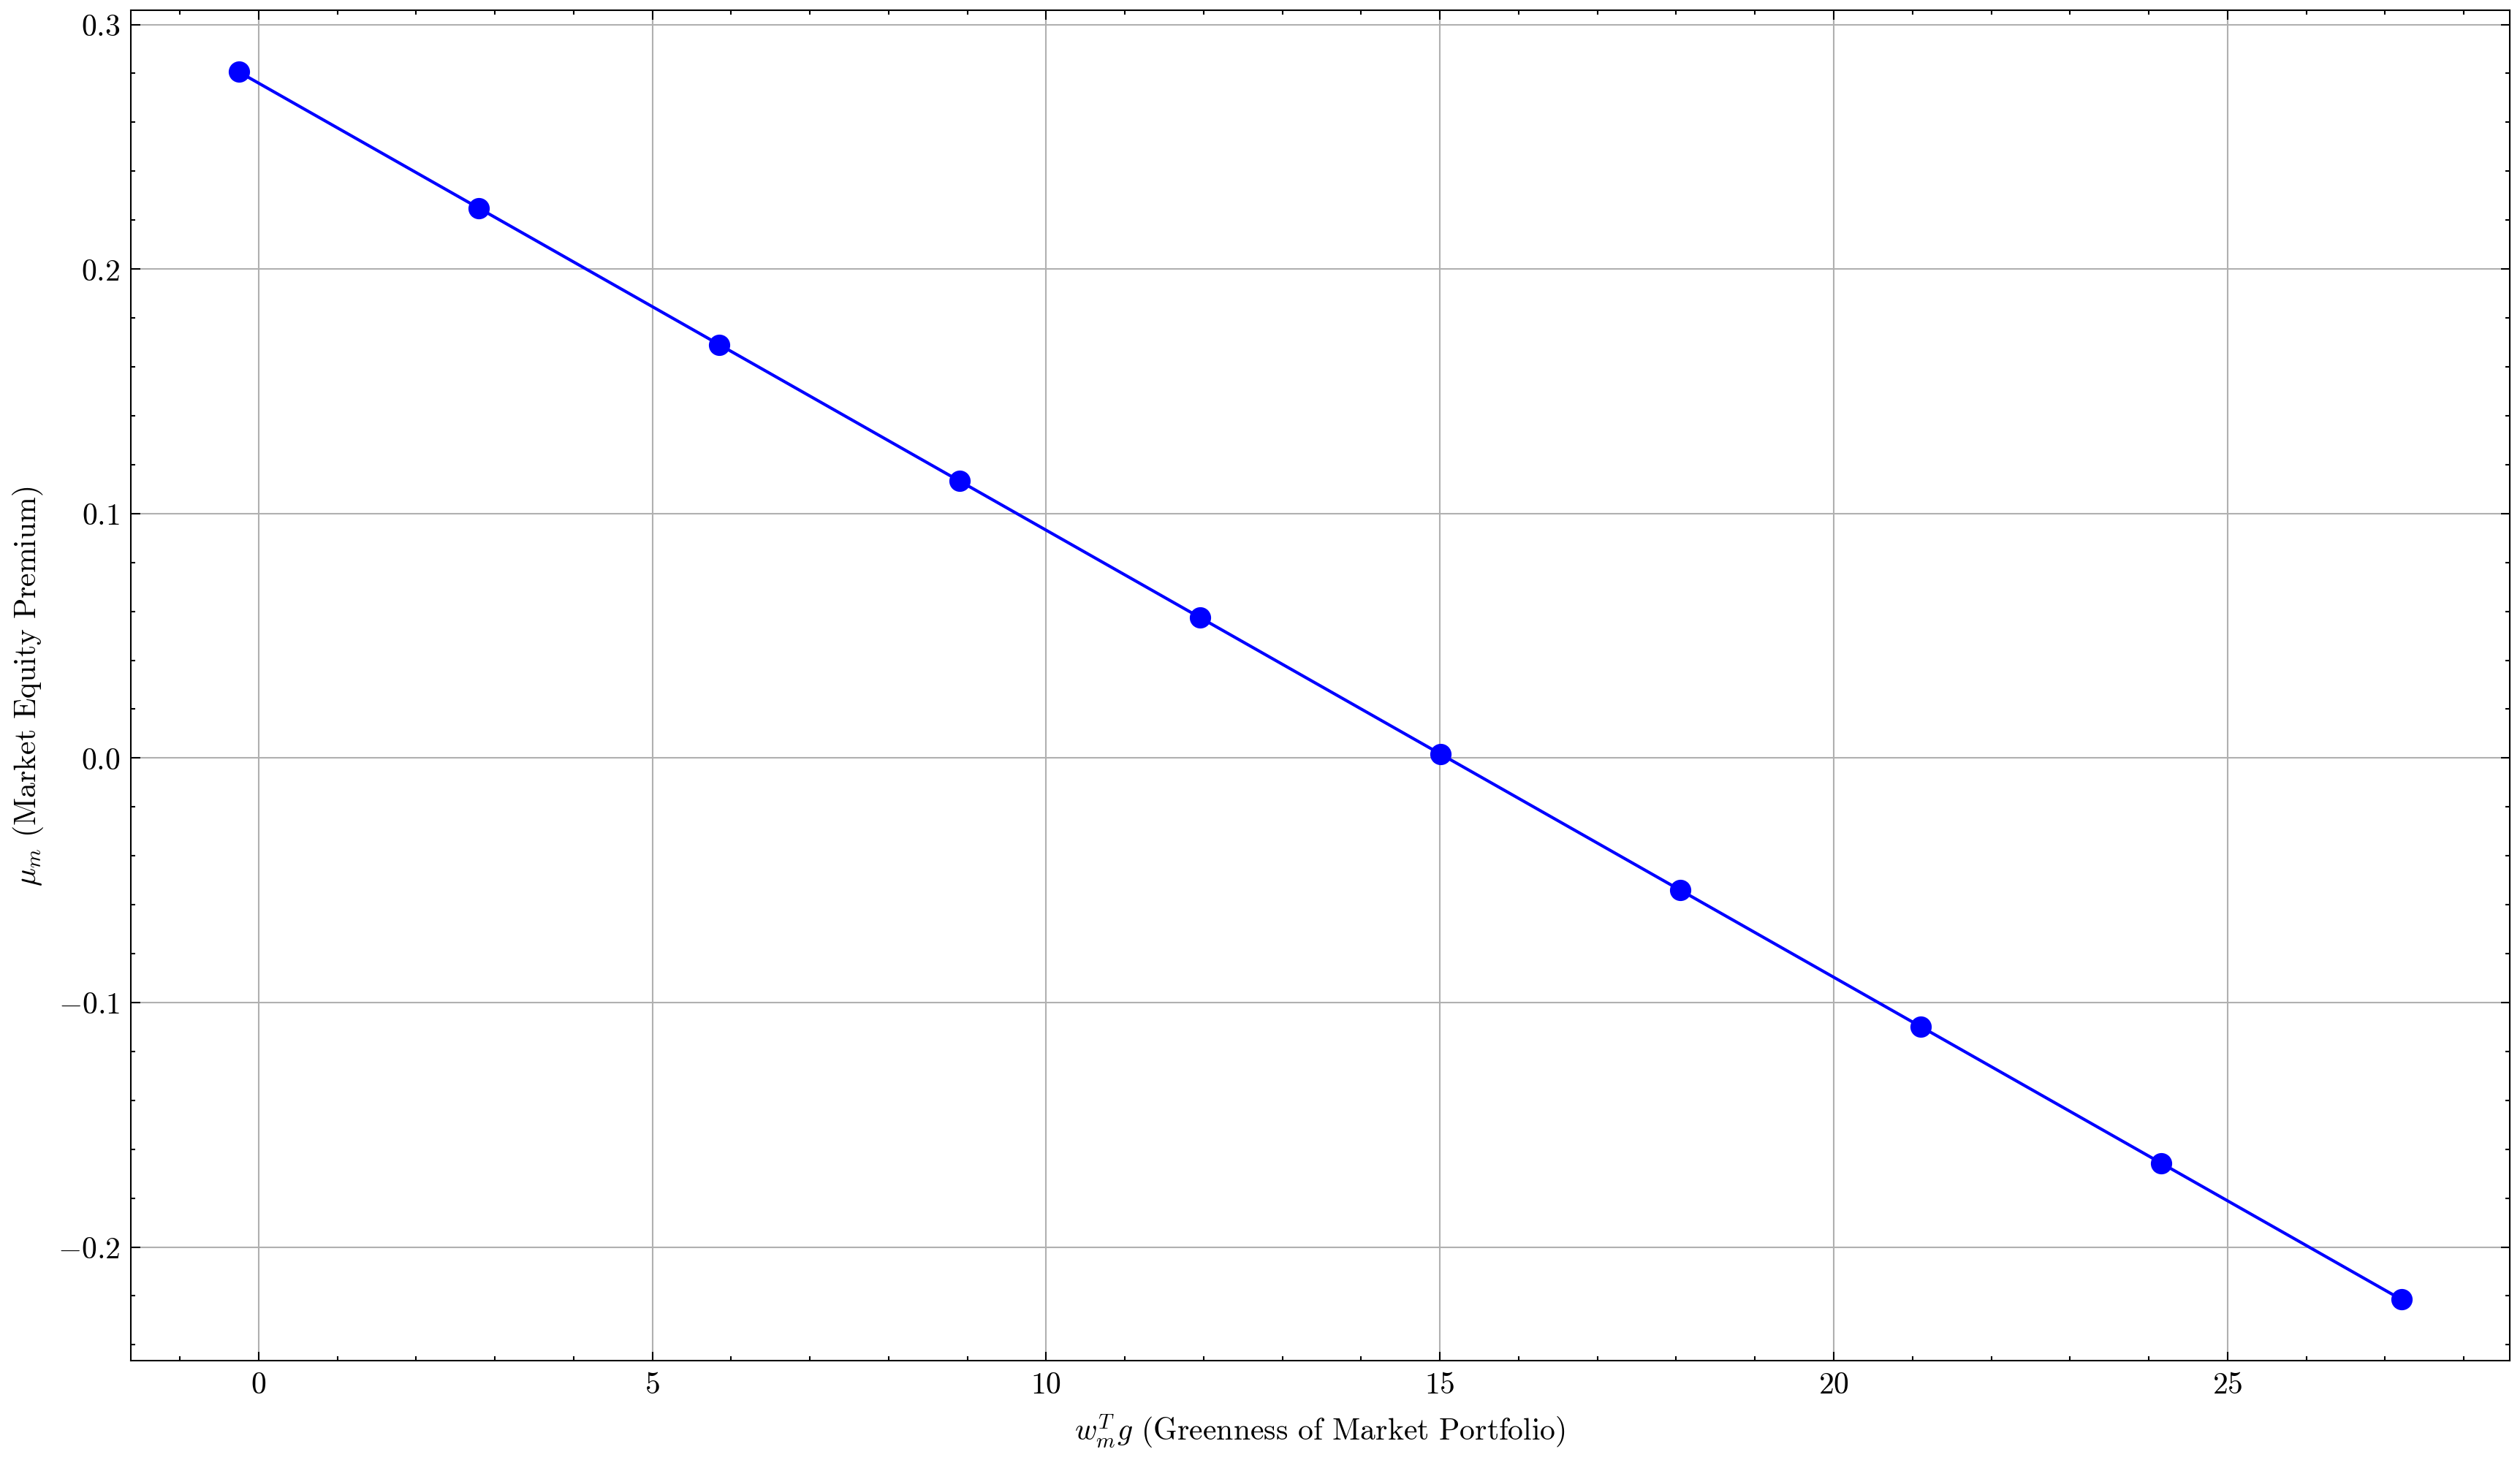
\includegraphics[width=1\textwidth]{../images/chapter01/market_equity_premium_vs_greenness.png}
    \caption{Market Equity Premium vs Market Greeness}
    \label{fig:equity_premium}
\end{figure}

The equity premium $\mu_m$ depends on the average of ESG tastes, $\bar{d}$,
through the "greeness" of the market portfolio $w_m^T g$.
If the market is net green (i.e., $w_m^T g > 0$), then stronger 
ESG tastes (higher $\bar{d}$) lead to lower equity premium.

Conversely, if the market is net "brown" ($w_m^T g < 0$), then stronger
ESG tastes lead to higher equity premium as investors demand 
compensation for holding brown stocks.


\subsection{Expected Excess Returns}

\subsubsection{Average Expected Excess Returns}

For simplicity, we assume that the market portfolio is ESG-neutral:

\begin{equation}
    w_m^T g = 0
\end{equation}

which implies that the equity premium is:

\begin{equation}
    \mu_m = a \sigma_m^2
\end{equation}

that is, independent of the average ESG tastes $\bar{d}$.

From the last equation, we note that $a = \frac{\mu_m}{\sigma_m^2}$, then 
the expected excess returns can be reexpressed as: 

\begin{equation}
    \begin{aligned}
        \mu = a \Sigma w_m - \frac{1}{a} g \bar{d} \\
        = \frac{\mu_m}{\sigma_m^2} \Sigma w_m - \frac{1}{a} g \bar{d} \\
        = \mu_m \beta_m - \frac{1}{a} g \bar{d} \\
    \end{aligned}
\end{equation}

where we have used the fact that the 
vector of market betas is $\beta_m = \frac{\Sigma w_m}{\sigma_m^2}$.

This gives the first proposition of the model:

\paragraph{Proposition 1.}
\textit{Expected excess returns in equilibirium are given by:}

\begin{equation}
    \mu = \mu_m \beta_m - \frac{\bar{d}}{a} g 
\end{equation}

\textit{
The expected excess returns deviate from their CAPM values due to ESG 
tastes for holding green stocks.}

\paragraph{Corrolary 1.}
\textit{If $\bar{d} > 0$, the expected return on stock $n$ is decreasing in $g_n$}.

\textit{Given their ESG tastes, agents are willing to pay more for greener firms, then 
lowering the firms' expected returns.}

\paragraph{Corrolary 2.} \textit{Because the vector of stocks' CAPM alphas is defined as 
$\alpha := \mu - \mu_m \beta_m$, we have:}

\begin{equation}
    \alpha_n = - \frac{\bar{d}}{a} g_n
\end{equation}

\textit{If $\bar{d} > 0$, green stocks have negative alphas, and brown stocks 
have positive alphas. Greener stocks have lower alphas.}


\begin{figure}
    \centering
    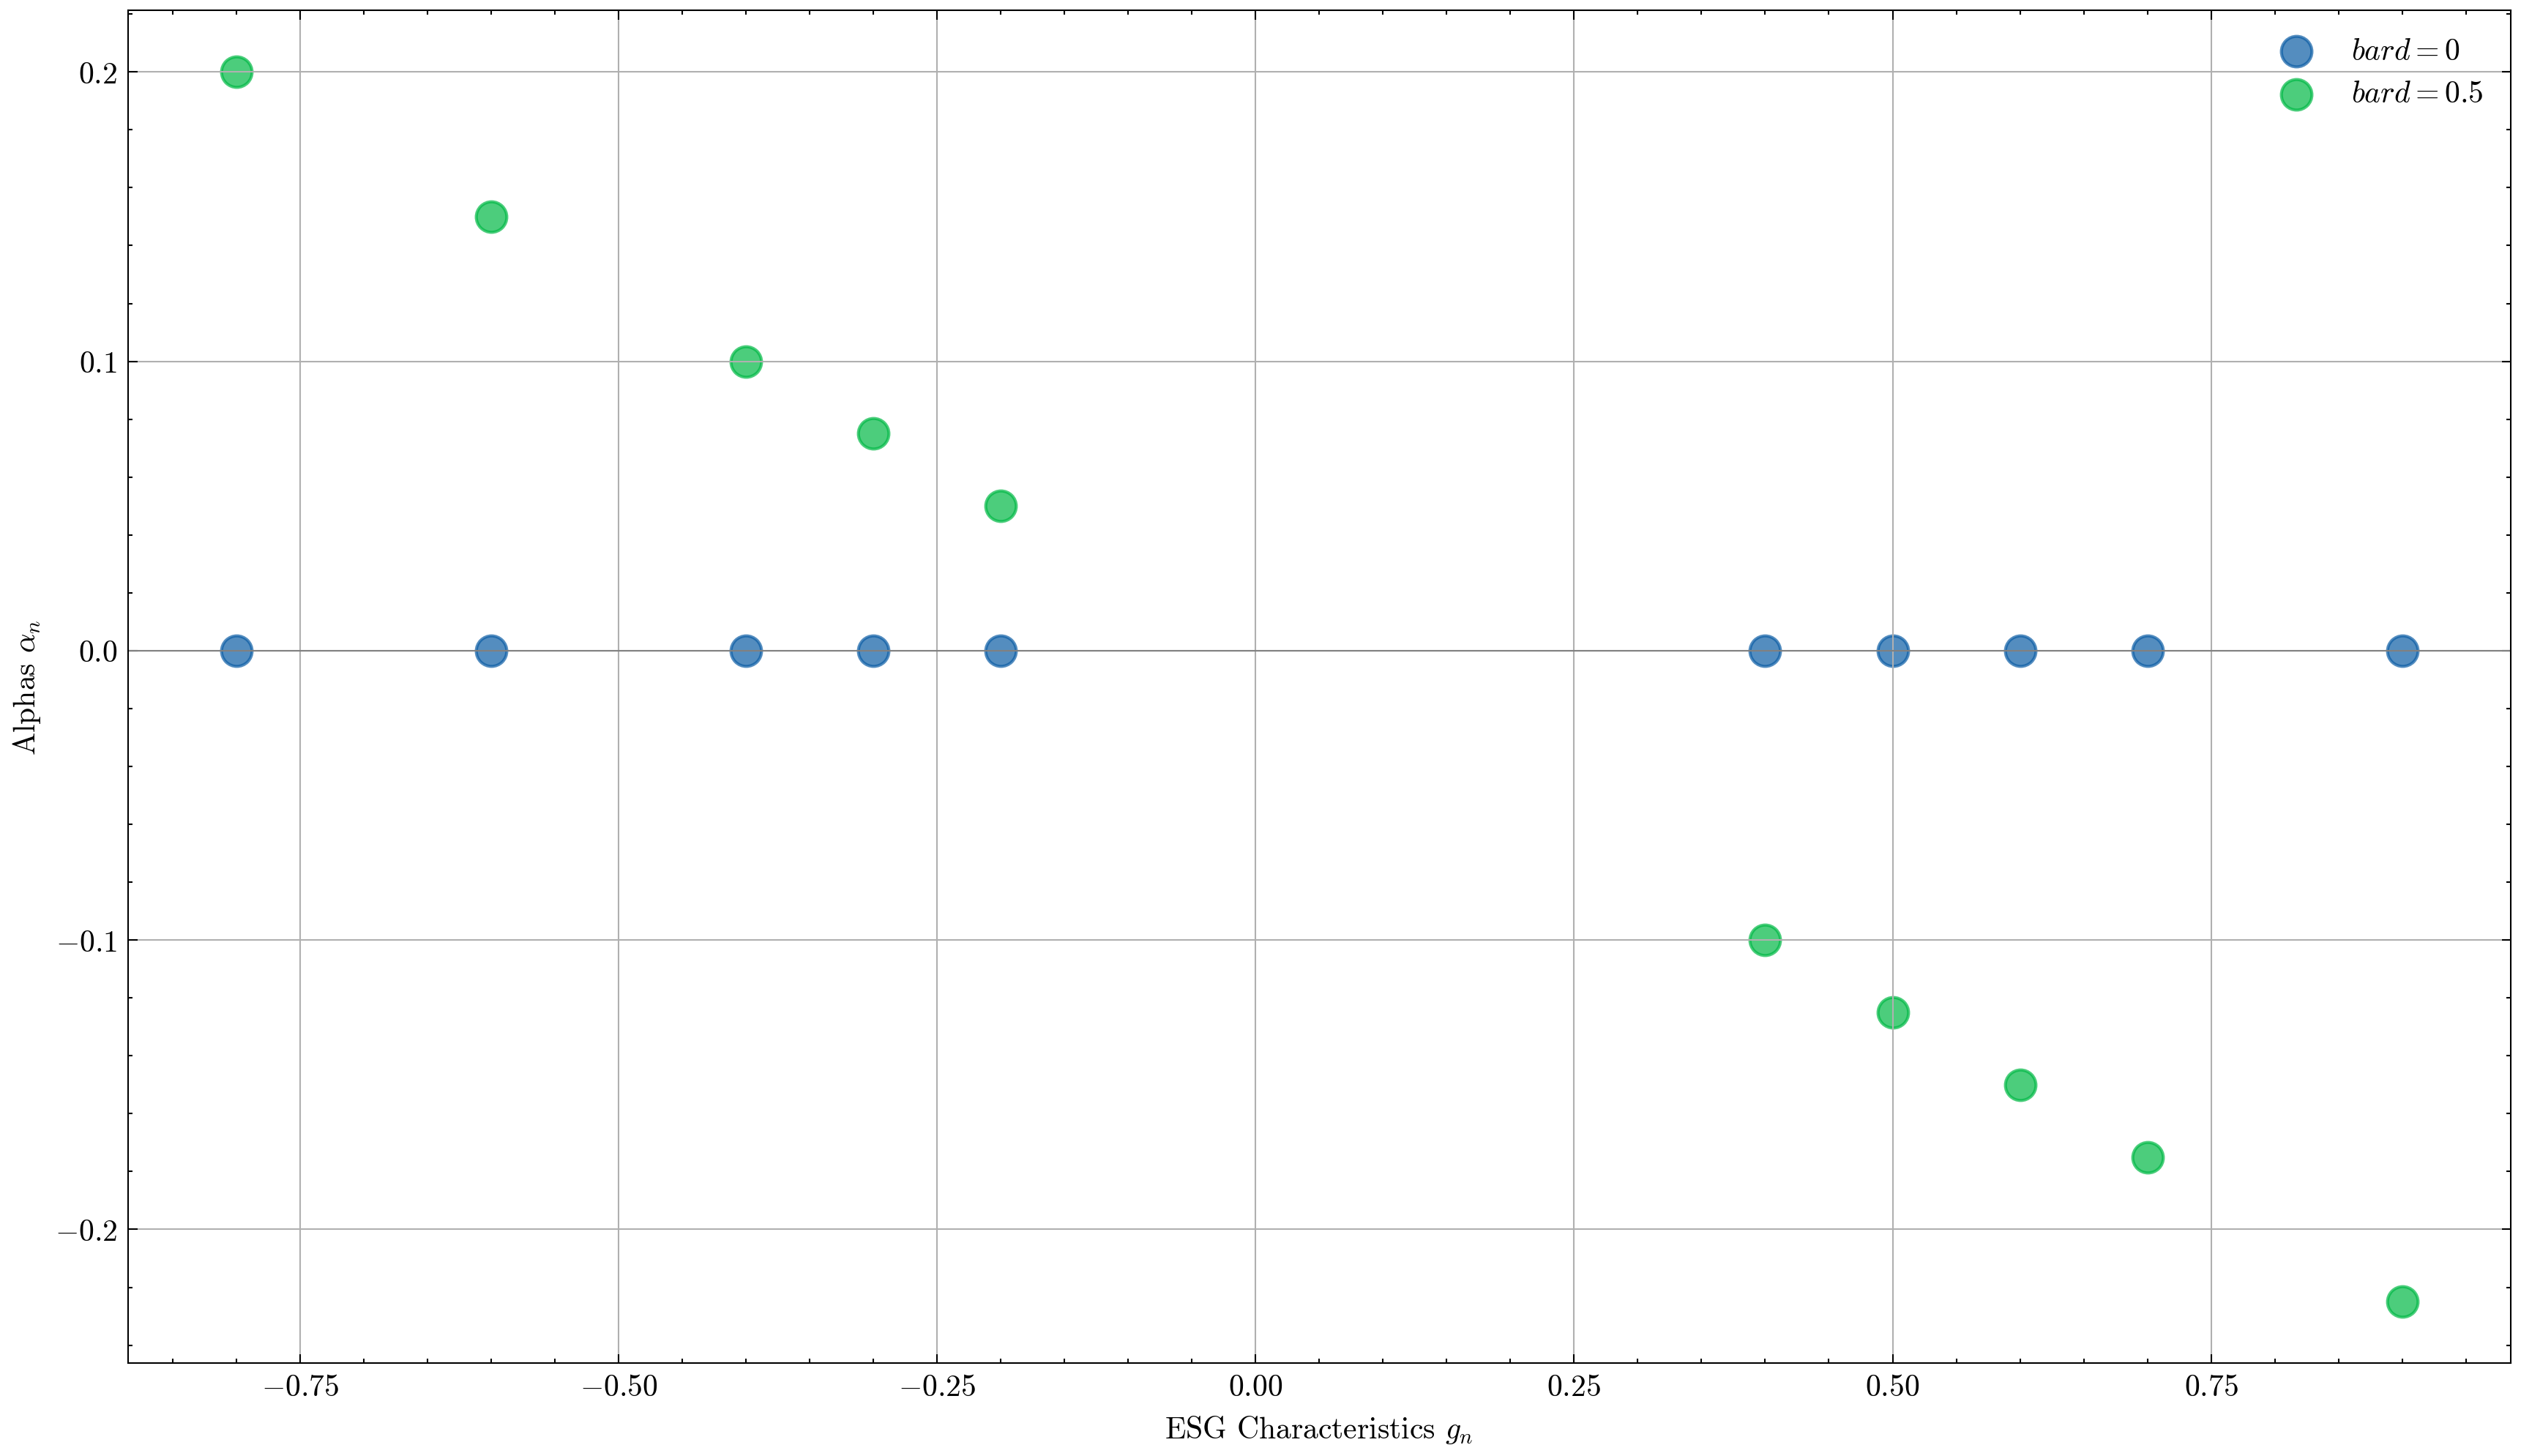
\includegraphics[width=1\textwidth]{../images/chapter01/alphas_vs_esg_characteristics.png}
    \caption{$\alpha_n$ relationship with $g_n$}
    \label{fig:esg_returns}
\end{figure}

\subsubsection{Investor $i$'s Excess Returns Mean and Variance}

Investor $i$'s expected excess return is given by:
\begin{equation}
    \begin{aligned}
E(\tilde{r}_{1,i}) = X_i^T \mu \\ 
    \end{aligned}
\end{equation}

We know that $\mu = \mu_m \beta_m - \frac{\bar{d}}{a} g$ from the Proposition 1:

\begin{equation}
    \begin{aligned}
E(\tilde{r}_{1,i}) = X_i^T (\mu_m \beta_m - \frac{\bar{d}}{a} g) \\
    \end{aligned}
\end{equation}

We can express $X_i$ in terms of $w_m$ by susbtracting the expression $w_m$ 
from the expression of $X_i$. Recall the assumption that $a_i = a$ and distribute:

\begin{equation}
    \begin{aligned}
        E(\tilde{r}_{1,i}) = (w_m^T + \frac{1}{a} \Sigma^{-1} (\mu + \frac{d_i}{a}g) - \frac{1}{a} \Sigma^{-1} \mu - \frac{\bar{d}}{a^2} \Sigma^{-1} g) (\mu_m \beta_m - \frac{\bar{d}}{a} g) \\
        = (w_m^T + \frac{1}{a} \Sigma^{-1}\mu - \frac{1}{a} \Sigma^{-1} \mu + \frac{d_i}{a^2}\Sigma^{-1}g - \frac{\bar{d}}{a^2} \Sigma^{-1}g)(\mu_m \beta_m - \frac{\bar{d}}{a}g)\\
        = (w_m^T + \frac{d_i - \bar{d}}{a^2} \Sigma^{-1} g) (\mu_m \beta_m - \frac{\bar{d}}{a} g) \\
    \end{aligned}
\end{equation}

Rewriting $d_i - \bar{d} = \delta_i$, recalling that $\beta_m = (\frac{1}{\sigma^2_m})\Sigma w_m$ and distribute:

\begin{equation}
    \begin{aligned}
        E(\tilde{r}_{1,i}) = (w_m^T + \frac{\delta_i}{a^2} \Sigma^{-1} g) (\frac{\mu_m}{\sigma^2_m} \Sigma w_m - \frac{\bar{d}}{a}g) \\
= w_m^T \frac{\mu_m}{\sigma^2_m} \Sigma w_m - w_m^T \frac{\bar{d}}{a} g + \frac{\delta_i \mu_m}{a^2\sigma^2_m}\Sigma^{-1}\Sigma g^T w_m - \frac{\delta_i \bar{d}}{a^3} g^T \Sigma g \\
= w_m^T \frac{\mu_m}{\sigma^2_m} \Sigma w_m - w_m^T \frac{\bar{d}}{a} g + \frac{\delta_i \mu_m}{a^2\sigma^2_m} g^T w_m - \frac{\delta_i \bar{d}}{a^3} g^T \Sigma g\\
    \end{aligned}
\end{equation}

We now that $w_m^T \Sigma w_m = \sigma^2_m$, so we have:

\begin{equation}
    \begin{aligned}
        E(\tilde{r}_{1,i}) = \mu_m - w_m^T \frac{\bar{d}}{a}g + \frac{\delta_i \mu_m}{a^2\sigma^2_m} g^T w_m - \frac{\delta_i \bar{d}}{a^3} g^T \Sigma g\\
    \end{aligned}
\end{equation}

Recalling the assumption that $w_m^T g = 0$, we finally have:
\begin{equation}
    \begin{aligned}
        E(\tilde{r}_{1,i}) = \mu_m  - \frac{\delta_i \bar{d}}{a^3} g^T \Sigma g\\
    \end{aligned}
\end{equation}


\paragraph{Proposition 2.} \textit{The mean of the excess return on 
investor $i$'s portfolio is given by:}

\begin{equation}
    E(\tilde{r}_{1,i}) = \mu_m - \frac{\delta_i \bar{d}}{a^3} g^T \Sigma g
\end{equation}

\textit{Investor $i$ with $\delta_i > 0$ accepts below-market expected returns 
in exchange for satisfying their stronger tastes for holding green stocks.
Conversely, and as a result, investor $i$ with $\delta_i < 0$ enjoys above-market expected returns.}


The variance of the excess return on investor $i$'s portfolio is:

\begin{equation}
    \text{Var}(\tilde{r}_{1,i}) = X_i^T \Sigma X_i
\end{equation}

Again, we can express $X_i$ in terms of $w_m$ by susbtracting the expression $w_m$
from the expression of $X_i$, then distribute:

\begin{equation}
    \begin{aligned}
        \text{Var}(\tilde{r}_{1,i}) = (w^T_m + \frac{\delta_i}{a^2} \Sigma^{-1}g) \Sigma (w^T_m + \frac{\delta_i}{a^2} \Sigma^{-1}g) \\
        = w^T_m \Sigma w_m + w^T_m \Sigma \frac{\delta_i}{a^2} \Sigma^{-1}g + w^T_m \Sigma \frac{\delta_i}{a^2} \Sigma^{-1}g + \frac{\delta_i^2}{a^4} g^T \Sigma^{-1} \Sigma \Sigma^{-1} g \\
        = w^T_m \Sigma w_m + w^T_m \frac{\delta_i}{a^2} g + w^T_m \frac{\delta_i}{a^2} g + \frac{\delta_i^2}{a^4} g^T \Sigma^{-1} g \\
    \end{aligned}
\end{equation}

Finally, we recall that $w^T_m \Sigma w_m = \sigma^2_m$ and the assumption 
that $w_m^T g = 0$, then we have:

\begin{equation}
    \begin{aligned}
        \text{Var}(\tilde{r}_{1,i}) = \sigma^2_m + \frac{\delta_i^2}{a^4} g^T \Sigma^{-1} g \\
    \end{aligned}
\end{equation}

\paragraph{Proposition 3.} \textit{The variance of the excess return on
investor $i$'s portfolio is given by:}

\begin{equation}
    \text{Var}(\tilde{r}_{1,i}) = \sigma^2_m + \frac{\delta_i^2}{a^4} g^T \Sigma^{-1} g
\end{equation}

\textit{In departing from the market portfolio, all agents with $\delta_i \neq 0$
incur higher volatility than that of the market portfolio.}

\subsection{Investor's Utility in Equilibrium}

The lower expected returns earned by ESG-oriented investors 
do not imply that these agents are unhappy. Indeed, 
the more an investor's ESG preferences $d_i$ differ from the 
average in either direction, the more 
ESG preferences contribute to the investor's utility.
To see this, we start again from the investor's expected utility:


\begin{equation}
    \begin{aligned}
    E_0(V(\tilde{W}_{1,i}, X_i)) = 
     -\exp{(-a_i (1 + r_f))} \exp{(-a_i X_i^T (\mu + \frac{b_i}{a_i})+\frac{1}{2}a_i^2 X_i^T \Sigma X_i)} \\
    \end{aligned}
\end{equation}

In the second exponent term, we know from the equation 
of the investor's expected excess returns that (and recalling the assumption $a_i = a$):

\begin{equation}
    \begin{aligned}
    -a_iX_i^T \mu = -a (\mu_m - \frac{\delta_i \bar{d}}{a^3} g^T \Sigma g) \\
    = -a \mu_m + \frac{\delta_i \bar{d}}{a^2} g^T \Sigma g
    \end{aligned}
\end{equation}

We have the term $-ai X_i^T \frac{b_i}{a_i} = -X_i^T b_i$, where we 
again can express $X_i$ in terms of $w_m$ and recall that $b_i = d_i g$ and 
the assumption that $w_m^T g = 0$:

\begin{equation}
    \begin{aligned}
    -X_i^T b_i = -X_i^T d_i g \\
    = - (w_m^T + \frac{\delta_i}{a^2} g^T \Sigma^{-1}) d_i g \\
    = -w_m^T d_i g - \frac{\delta_i}{a^2} g^T \Sigma^{-1} d_i g \\
    = - \frac{\delta_i}{a^2} g^T \Sigma^{-1} d_i g
    \end{aligned}
\end{equation}

And we have finally the term $\frac{1}{2}a_i^2 X_i^T \Sigma X_i$,
where we recognize $X_i^T \Sigma X_i$ that we have found earlier:

\begin{equation}
    \begin{aligned}
    \frac{1}{2}a_i^2 X_i^T \Sigma X_i = \frac{1}{2}a_i^2 (w_m^T + \frac{\delta_i}{a^2} g^T \Sigma^{-1}) \Sigma (w_m + \frac{\delta_i}{a^2} g^T \Sigma^{-1}) \\
        = \frac{a^2}{2}(\sigma^2_m + \frac{\delta_i^2}{a^4} g^T \Sigma^{-1} g) \\
        = \frac{a^2}{2} \sigma^2_m + \frac{\delta_i^2}{2a^2} g^T \Sigma^{-1} g
    \end{aligned}
\end{equation}

Adding the three terms together, we have:

\begin{equation}
    \begin{aligned}
        -a_i X^T \mu - X_i^T b_i + (\frac{a^2}{2})X_i^T \Sigma X_i \\
        = -a \mu_m + \frac{\delta_i \bar{d}}{a^2} g^T \Sigma g -  \frac{\delta_i}{a^2} g^T \Sigma^{-1} d_i g + \frac{a^2}{2} \sigma^2_m + \frac{\delta_i^2}{2a^2} g^T \Sigma^{-1} g \\
    \end{aligned}
\end{equation}

We can factorize with $\frac{1}{a^2}$ and $g^T \Sigma g$:

\begin{equation}
    \begin{aligned}
        -a \mu_m + \frac{\delta_i \bar{d}}{a^2} g^T \Sigma g -  \frac{\delta_i}{a^2} g^T \Sigma^{-1} d_i g + \frac{a^2}{2} \sigma^2_m + \frac{\delta_i^2}{2a^2} g^T \Sigma^{-1} g \\
        = -a \mu_m + \frac{a^2}{2} \sigma^2_m + \frac{1}{a^2} ( \delta_i \bar{d} - \delta_i d_i + \frac{\delta_i^2}{2}) g^T \Sigma g\\
    \end{aligned}
\end{equation}

with $\delta_i \bar{d} - d_i \delta_i = (d_i - \bar{d})\delta_i = \delta_i^2$ and 
factorizing with $-a$ we have:

\begin{equation}
    \begin{aligned}
        -a \mu_m + \frac{a^2}{2} \sigma^2_m + \frac{1}{a^2} ( \delta_i \bar{d} - \delta_i d_i + \frac{\delta_i^2}{2}) g^T \Sigma g = -a(\mu_m + \frac{a}{2}\sigma^2_m) - \frac{\delta_i^2}{2a^2}g^T \Sigma^{-1} g\\
    \end{aligned}
\end{equation}

Substituting this into the utility function we have:

\begin{equation}
    \begin{aligned}
        E_0(V(\tilde{W}_{1,i}, X_i)) = -\exp{(-a(1 + r_f))} \exp{(-a(\mu_m + \frac{a}{2}\sigma^2_m) - \frac{\delta_i^2}{2a^2}g^T \Sigma^{-1} g)} \\
    \end{aligned}
\end{equation}

We can separate the terms related with $\delta_i$: 

\begin{equation}
    \begin{aligned}
        E_0(V(\tilde{W}_{1,i}, X_i)) = (-\exp{(-a(1 + r_f))} \exp{(-a(\mu_m + \frac{a}{2}\sigma^2_m))}) \exp{(-\frac{\delta_i^2}{2a^2}g^T \Sigma^{-1} g)} \\
        = \bar{V} \exp{(-\frac{\delta_i^2}{2a^2}g^T \Sigma^{-1} g)} \\
    \end{aligned}
\end{equation}

If the investor's ESG preferences are on the average, then $\delta_i = 0$ and
the investor's utility is $\bar{V}$. The expected utility 
is increasing in $\delta_i^2$, so the more an agent's ESG preferences 
differ from the average in either direction, the more ESG preferences
contributes to the agent's utility.


\begin{figure}
    \centering
    PLACEHOLDER
    % \includegraphics[width=0.8\textwidth]{images/ESG_taste.png}
    \caption{Investor's Utility with ESG Preferences}
    \label{fig:esg_utility}
\end{figure}

\newpage
\section{ESG Portfolio}

\subsection{Portfolio Tilts}

We want to reexpress the 
investor's optimal portfolio weights $X_i$ in terms of 
the ESG characteristics $g$.

Plugging excess returns $\mu = a \Sigma w_m - \frac{\bar{d}}{a}$ 
into the investor's optimal portfolio weights $X_i = \frac{1}{a} \Sigma^{-1}(\mu + \frac{d_i}{a}g)$,
we get
the portfolio weights $X_i$ as a function of the ESG characteristics $g$ and the investor's
taste for ESG benefits $d_i$:

\begin{equation}
    \begin{aligned}
    X_i = \frac{1}{a} \Sigma^{-1}(\mu + \frac{d_i}{a}g) \\
     = \frac{1}{a} \Sigma^{-1}\mu + \frac{1}{a^2} \Sigma^{-1} g d_i \\
     = \frac{1}{a} \Sigma^{-1} (a \Sigma w_m - \frac{\bar{d}}{a} g) + \frac{1}{a^2} \Sigma^{-1} g d_i \\
     = \frac{1}{a}a\Sigma^{-1}\Sigma w_m - \frac{\bar{d}}{a^2} \Sigma^{-1} g + \frac{1}{a^2} \Sigma^{-1} g d_i \\
     = w_m - \frac{\bar{d}}{a^2} \Sigma^{-1} g + \frac{d_i}{a^2} \Sigma^{-1} g \\
        = w_m + \frac{d_i - \bar{d}}{a^2} \Sigma^{-1} g \\
    = w_m + \frac{\delta_i}{a^2} \Sigma^{-1} g
    \end{aligned}
\end{equation}

Therefore, we have a new proposition:

\paragraph{Proposition 4.} \textit{Investor $i$'s 
optimal portfolio weights on the $N$ stocks are given by:}

\begin{equation}
    X_i = w_m + \frac{\delta_i}{a^2} \Sigma^{-1} g
\end{equation}

This proposition implies three-fund separation, 
as each investor's portfolio can be implemented with three 
assets: (i) the risk-free asset, 
(ii) the market portfolio, and (iii) the ESG portfolio.
The ESG portfolio weights are proportional 
to $\Sigma^{-1} g$. 
The fraction of an investor $i$'s wealth in 
the risk-free asset, $1 - \mathbf{1}^T X_i = - (\delta_i/a^2)\mathbf{1}^T \Sigma^{-1}g$, 
can be positive or negative. 
The investor's remaining wealth is invested 
in stocks. Specifically, 
the investor allocates a fraction $\phi_i$ 
of her remaining wealth to the ESG portfolio,
and a fraction $1 - \phi_i$ to the market portfolio.

To see this, we note that the $N \times 1$ vector 
of weights within investor $i$'s stock portfolio $w_i$ is
$X_i$ normalized by the sum of its elements:

\begin{equation}
    \begin{aligned}
        w_i = X_i / \mathbf{1}^T X_i \\
        = \frac{w_m + \frac{\delta_i}{a^2} \Sigma^{-1} g}{\mathbf{1}^T (w_m + \frac{\delta_i}{a^2} \Sigma^{-1} g)} \\
    \end{aligned}
\end{equation}

We can expand the denominator:

\begin{equation}
    \begin{aligned}
        \mathbf{1}^T (w_m + \frac{\delta_i}{a^2} \Sigma^{-1} g) = \mathbf{1}^T w_m + \frac{\delta_i}{a^2} \mathbf{1}^T \Sigma^{-1} g \\
        = 1 + \frac{\delta_i}{a^2} \mathbf{1}^T \Sigma^{-1} g\\
    \end{aligned}
\end{equation}

because $\mathbf{1}^T w_m = 1$.
Substitute back into the normalization formula
and separate the terms in the numerator:

\begin{equation}
    \begin{aligned}
        w_i = \frac{w_m + \frac{\delta_i}{a^2} \Sigma^{-1} g}{1 + \frac{\delta_i}{a^2} \mathbf{1}^T \Sigma^{-1} g} \\
        = \frac{w_m}{1 + \frac{\delta_i}{a^2} \mathbf{1}^T \Sigma^{-1} g} + \frac{\frac{\delta_i}{a^2} \Sigma^{-1} g}{1 + \frac{\delta_i}{a^2} \mathbf{1}^T \Sigma^{-1} g} \\
    \end{aligned}
\end{equation}

Using the identity $\frac{1}{1 + x} = 1 - \frac{x}{1 + x}$, 
with $x = \frac{\delta_i}{a^2} \mathbf{1}^T \Sigma^{-1} g$,
we can rewrite 
the first term:

\begin{equation}
    \begin{aligned}
        \frac{w_m}{1 + \frac{\delta_i}{a^2} \mathbf{1}^T \Sigma^{-1} g} = w_m (1 - \frac{\delta_i / a^2 \mathbf{1}^T \Sigma^{-1}g}{1 + \delta_i / a^2 \mathbf{1}^T \Sigma^{-1}g}) \\
    \end{aligned}
\end{equation}

We put it back into the formula for $w_i$:

\begin{equation}
    \begin{aligned}
        w_i = w_m (1 - \frac{\delta_i / a^2 \mathbf{1}^T \Sigma^{-1}g}{1 + \delta_i / a^2 \mathbf{1}^T \Sigma^{-1}g}) + \frac{\delta_i / a^2 \Sigma^{-1}g}{1 + \delta_i / a^2 \mathbf{1}^T \Sigma^{-1}g} \\
        \end{aligned}
\end{equation}

$\Sigma^{-1}g$ must be normalized to sum to 1:

\begin{equation}
    w_g = \frac{1}{\mathbf{1}^T \Sigma^{-1} g} \Sigma^{-1} g
\end{equation}

So we can rewrite the second term as:

\begin{equation}
    \begin{aligned}
        w_i = w_m (1 - \frac{\delta_i / a^2 \mathbf{1}^T \Sigma^{-1}g}{1 + \delta_i / a^2 \mathbf{1}^T \Sigma^{-1}g}) + \frac{\delta_i / a^2}{1 + \delta_i / a^2 \mathbf{1}^T \Sigma^{-1}g} w_g \\
        = w_m \phi_i + w_g (1 - \phi_i) \\
    \end{aligned}
\end{equation}


with $\phi_i = \frac{\delta_i / a^2 \mathbf{1}^T \Sigma^{-1}g}{1 + \delta_i / a^2 \mathbf{1}^T \Sigma^{-1}g}$.

\begin{figure}
    \centering
    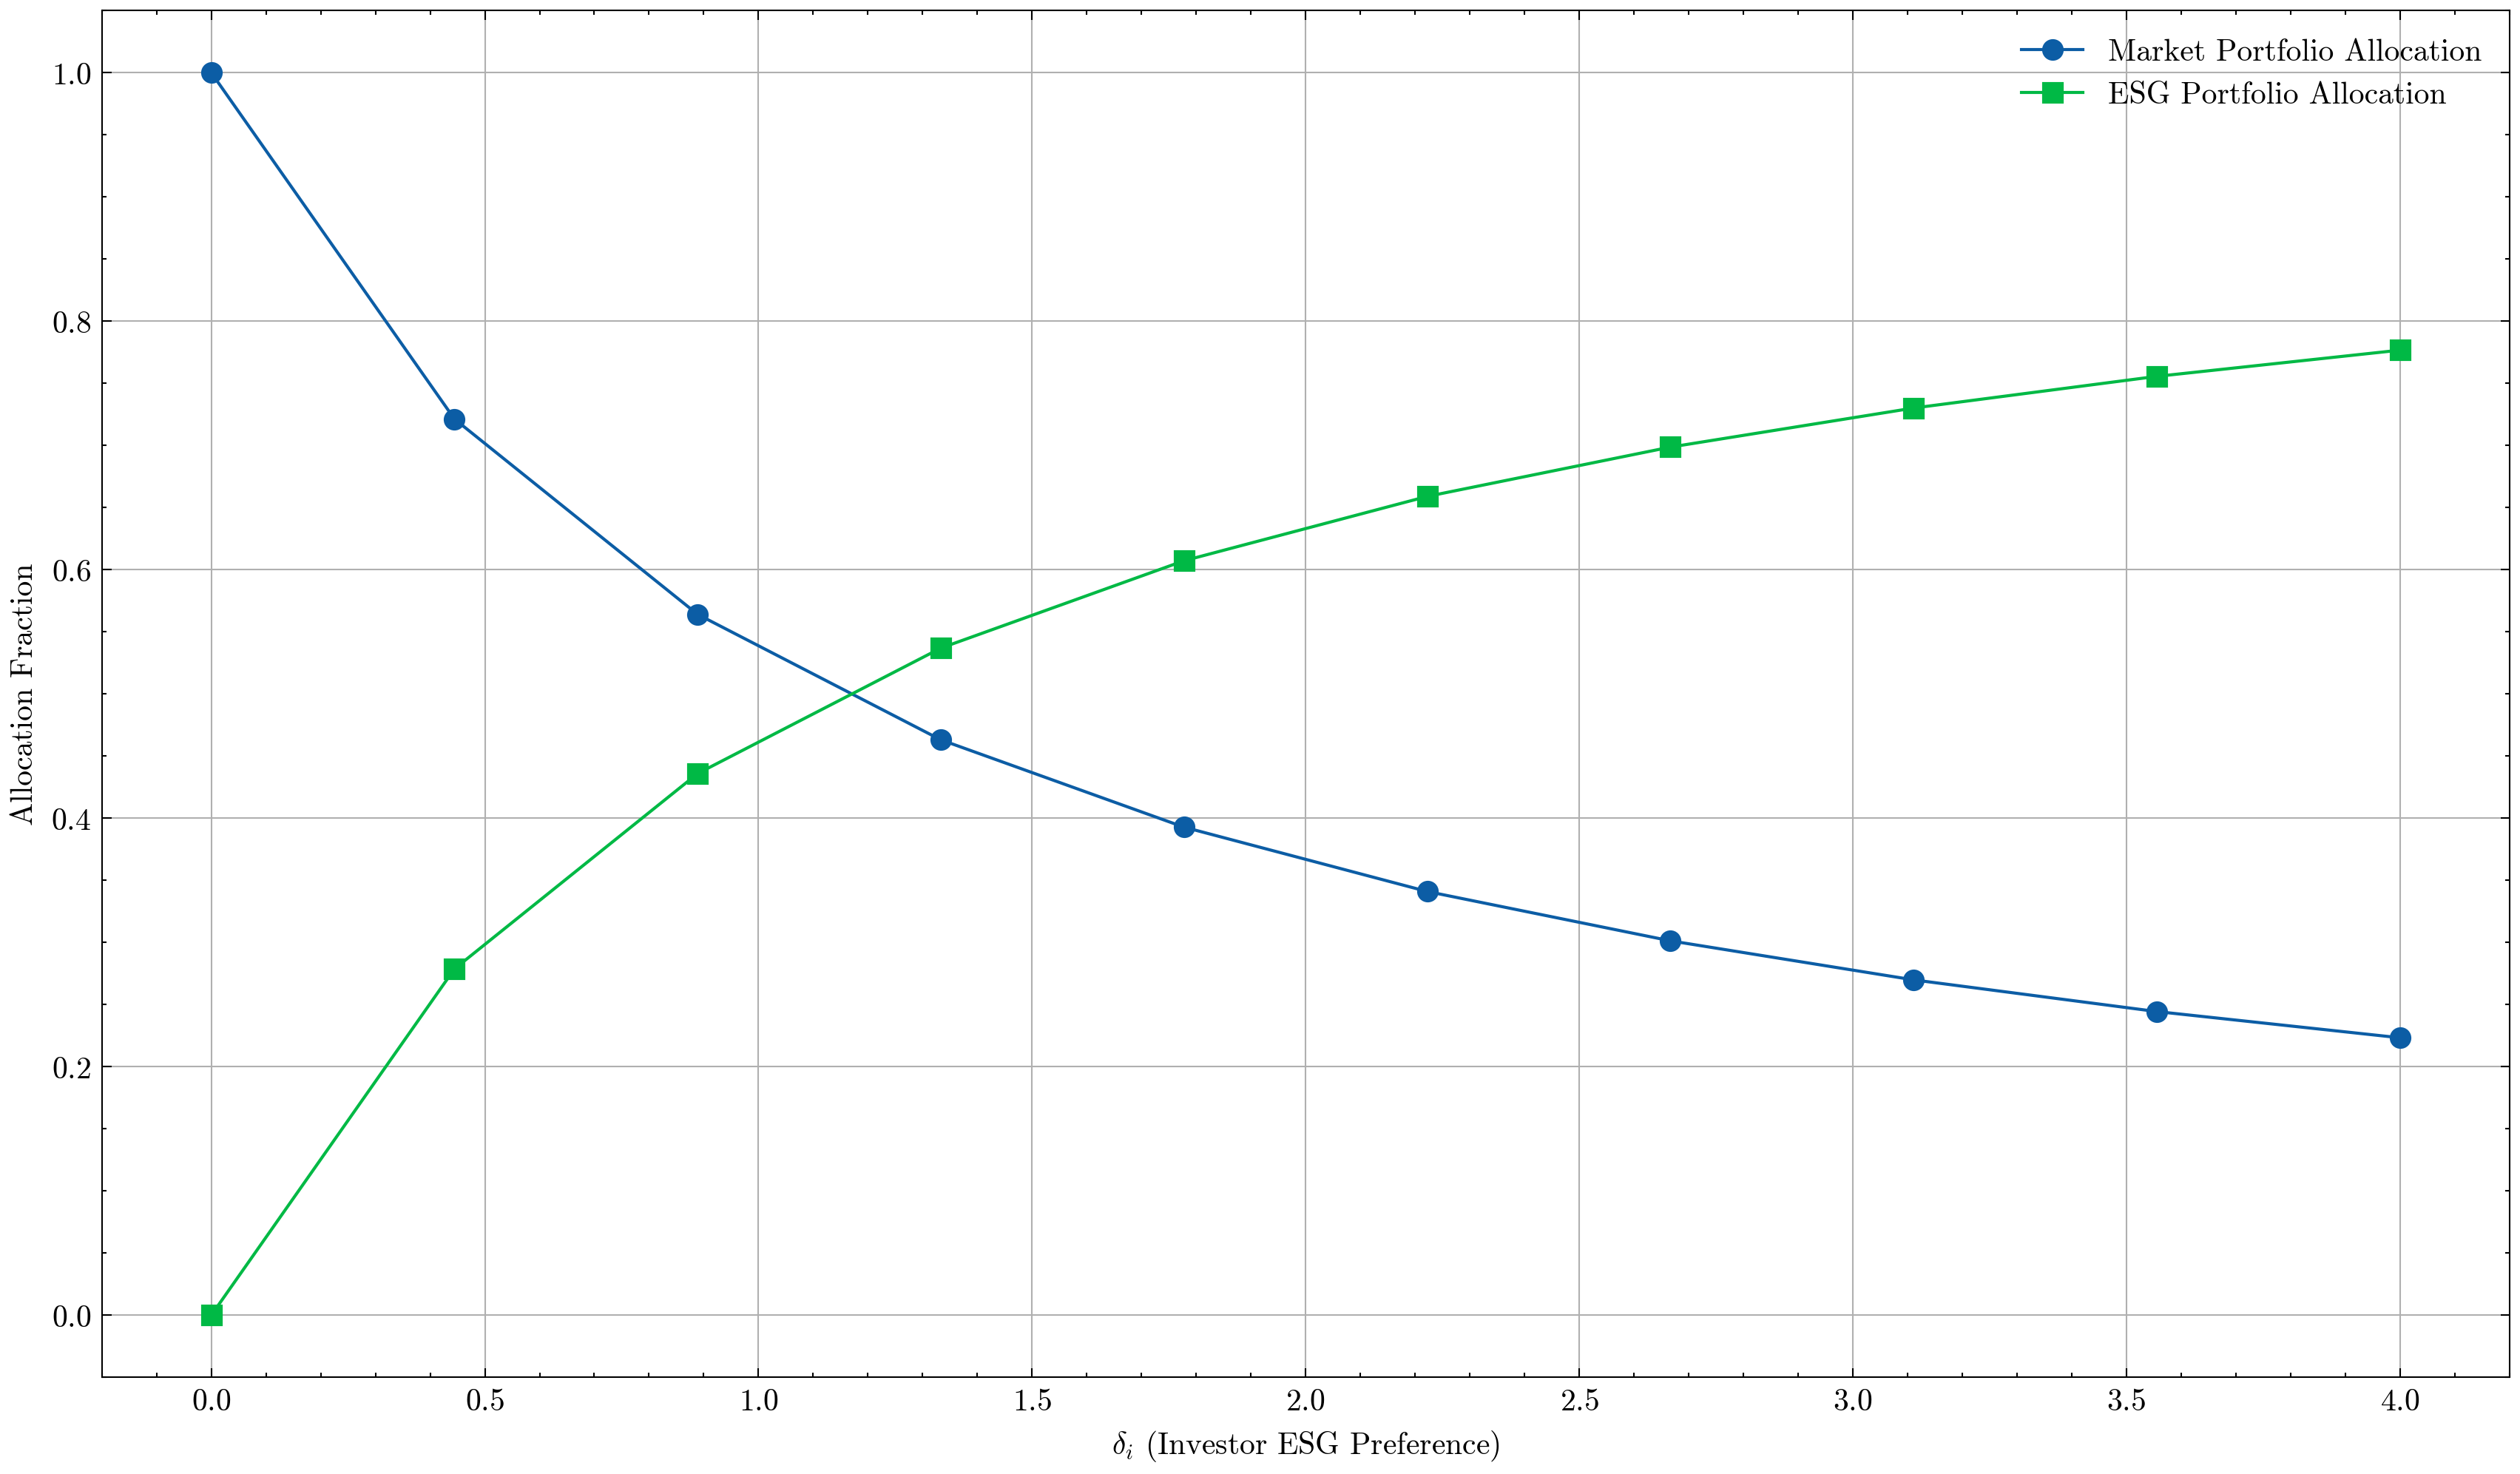
\includegraphics[width=1\textwidth]{../images/chapter01/allocation_fractions_vs_delta_i.png}
    \caption{Allocation Between Market and ESG Portfolio According to $\delta_i$,
    with $\delta_i \geq 0$}
    \label{fig:portfolio_tilts}
\end{figure}

In the special case where $\mathbf{1}^T \Sigma^{-1} g = 0$,
no investor holds the risk-free asset, and the ESG 
portfolio is a zero-cost position with:

\begin{equation}
    w_g = \Sigma^{-1} g
\end{equation}

so that: 

\begin{equation}
    w_i = w_m + \phi_i \Sigma^{-1} g
\end{equation}

where $\phi_i = \delta_i / a^2$.    

We denote the ESG portfolio greeness as: 

\begin{equation}
    g_g = w_g^T g 
\end{equation}

From the equation above, $g_g$ is nonzero as long as 
$g \neq 0$. Also, 
$g_g$ is negative if $\mathbf{1}^T \Sigma^{-1} g < 0$,
but it is otherwise positive. We see that $\phi_i$ 
has the same sign as the product of $\delta_i$ and $g_g$,
if the denominator of $\phi_i$ is positive (that is, 
if investor $i$ invests a positive fraction 
of her wealth in stocks, so that $\mathbf{1}^T X_i > 0$).

Therefore, for an investor with positive wealth 
in stocks and $\delta_i > 0$, $\phi_i$ is positive 
(negative) if $g_g$ is positive (negative).
That is, such an investor tilts away from 
the market portfolio in the direction of greeness,
that is she tilts towards the ESG portfolio 
when it is green and away from it when it is brown.
Applying our previous result, the 
ESG portfolio CAPM alpha is given by: 

\begin{equation}
    \alpha_g = - \frac{\bar{d}}{a} g_g
\end{equation}

whose sign is opposite to that of $g_g$. Therefore, 
investors with positive (negative) value of $\delta_i$
have ESG portfolios tilts that produce 
negative (positive) alphas for their overall portfolios.

The ESG tilt is zero (ie, $\phi_i = 0$) for 
investors with average ESG tastes ($\delta_i = 0$).
Those investors hold the market portfolio. In contrast,
investors who are indifferent to ESG ($d_i = 0$, thus 
$\delta_i < 0$) tilt away from the market portfolio.
In a world with ESG concerns, investors indifferent 
to ESG should tilt away from the market portfolio.
Otherwise they are not optimizing. The market portfolio
is optimal for investors with average ESG tastes.

\begin{figure}
    \centering
    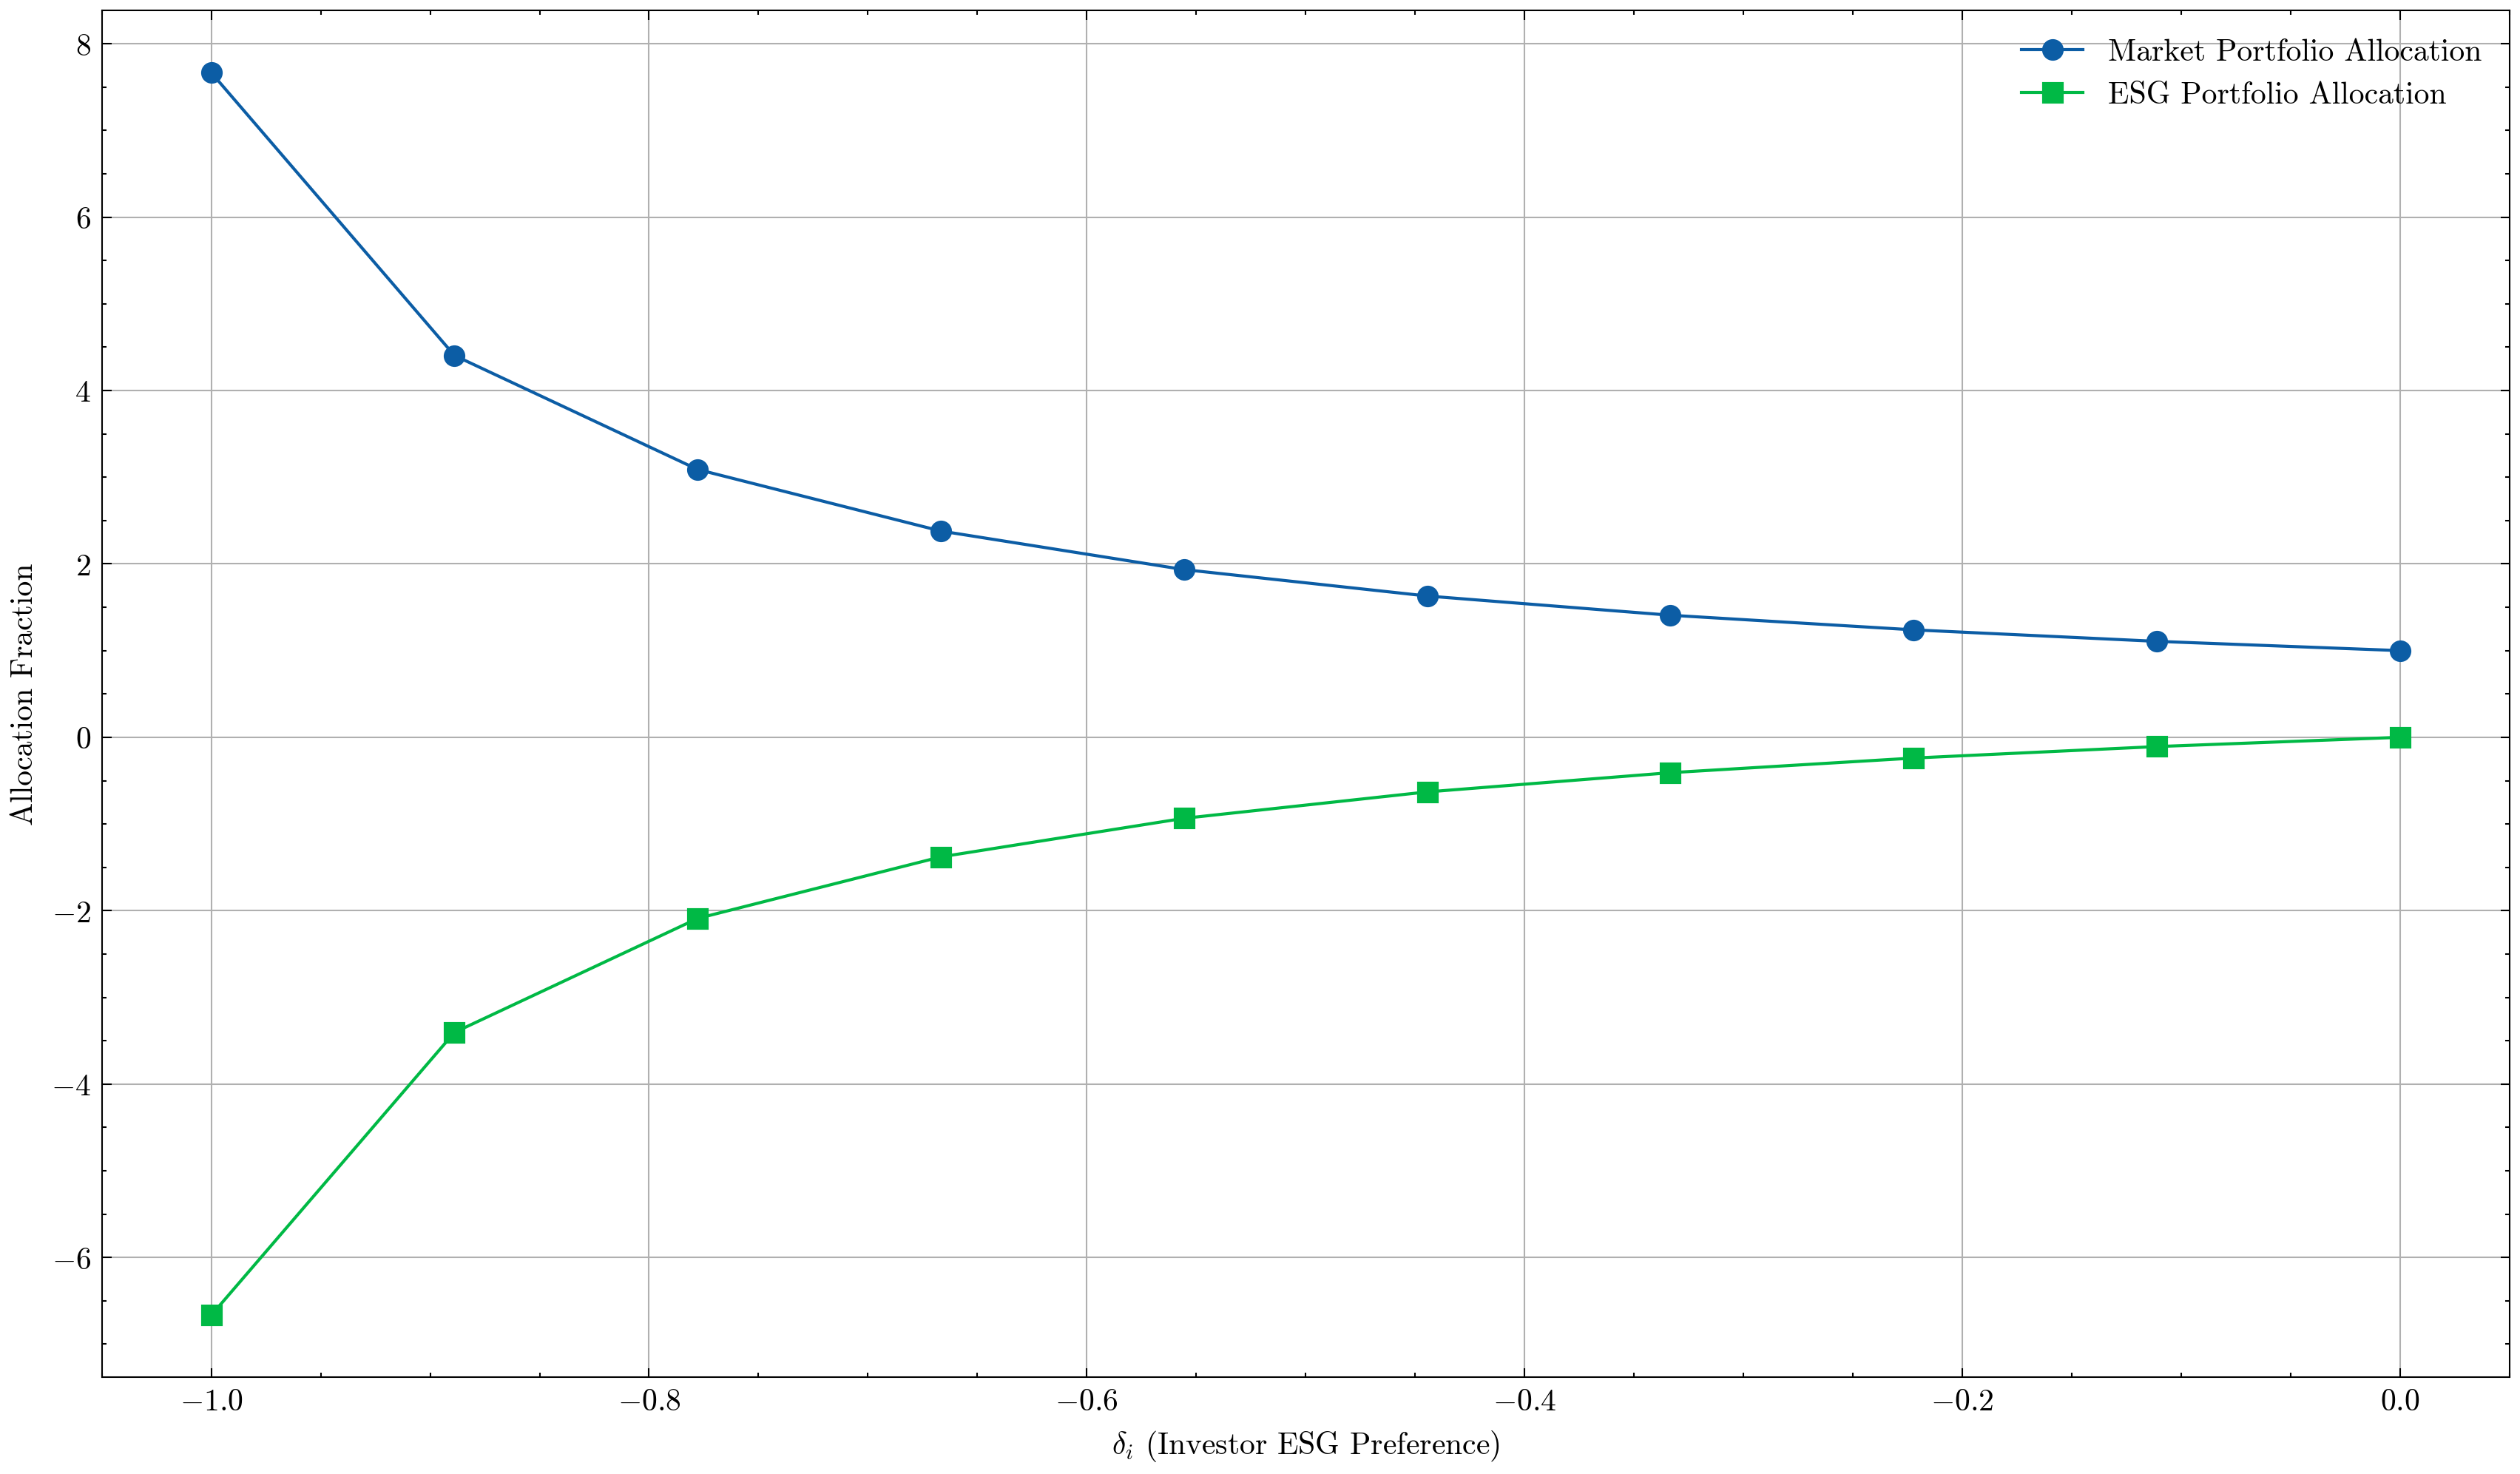
\includegraphics[width=1\textwidth]{../images/chapter01/allocation_fractions_vs_delta_i_short.png}
    \caption{Allocation Between Market and ESG Portfolio According to $\delta_i$,
    with $\delta_i < 0$}
    \label{fig:portfolio_tilts_short}
\end{figure}

If all agents have identical ESG concerns,
so that $\delta_i = 0$ for all $i$, 
then there is zero ESG tilt for each investor.
We thus have the following corrolary:

\paragraph{Corrolary 3.} \textit{If there is no 
dispertion in ESG tastes across investors, 
then all investors hold the market portfolio.}

All investors hold the market portfolio 
when none of them have ESG concerns, as in the 
standard CAPM. All agents also hold the market 
portfolio when all of them have the same ESG concerns.
The reason is that stock prices then fully adjust 
to reflect those tastes, again making the 
market everybody's optimal choice. Dispersion in 
ESG tastes is necessary for an ESG industry to exist.


\subsection{Factor Pricing with the ESG Portfolio}